\documentclass[11pt]{article}
\newcommand\floor[1]{\lfloor#1\rfloor}
\usepackage{amsmath}

%\usepackage{customizations}
\usepackage{listings}


\textwidth=15cm
\oddsidemargin=0.7cm
\voffset=-1cm
\textheight=20cm
\usepackage{xcolor}

\usepackage{graphicx}
\graphicspath{ {img/} }

\begin{document}

\title{
  CS 171: Visualization \\
  \Large{Homework 4 (Due October 2nd, 2017 at 11:59pm)}
}
\date{}

\maketitle

\vspace{-1cm}


\section*{Design Analysis / Critique}

\begin{enumerate}
  \item \textbf{Formulate Three Questions}
  \begin{enumerate}
    \item Which country has the best (lowest) gender inequality index?
    \item Which country has the lowest percentage of share of seats in parliament?
    \item Which continent has the lowest human development rate?
  \end{enumerate}
  
  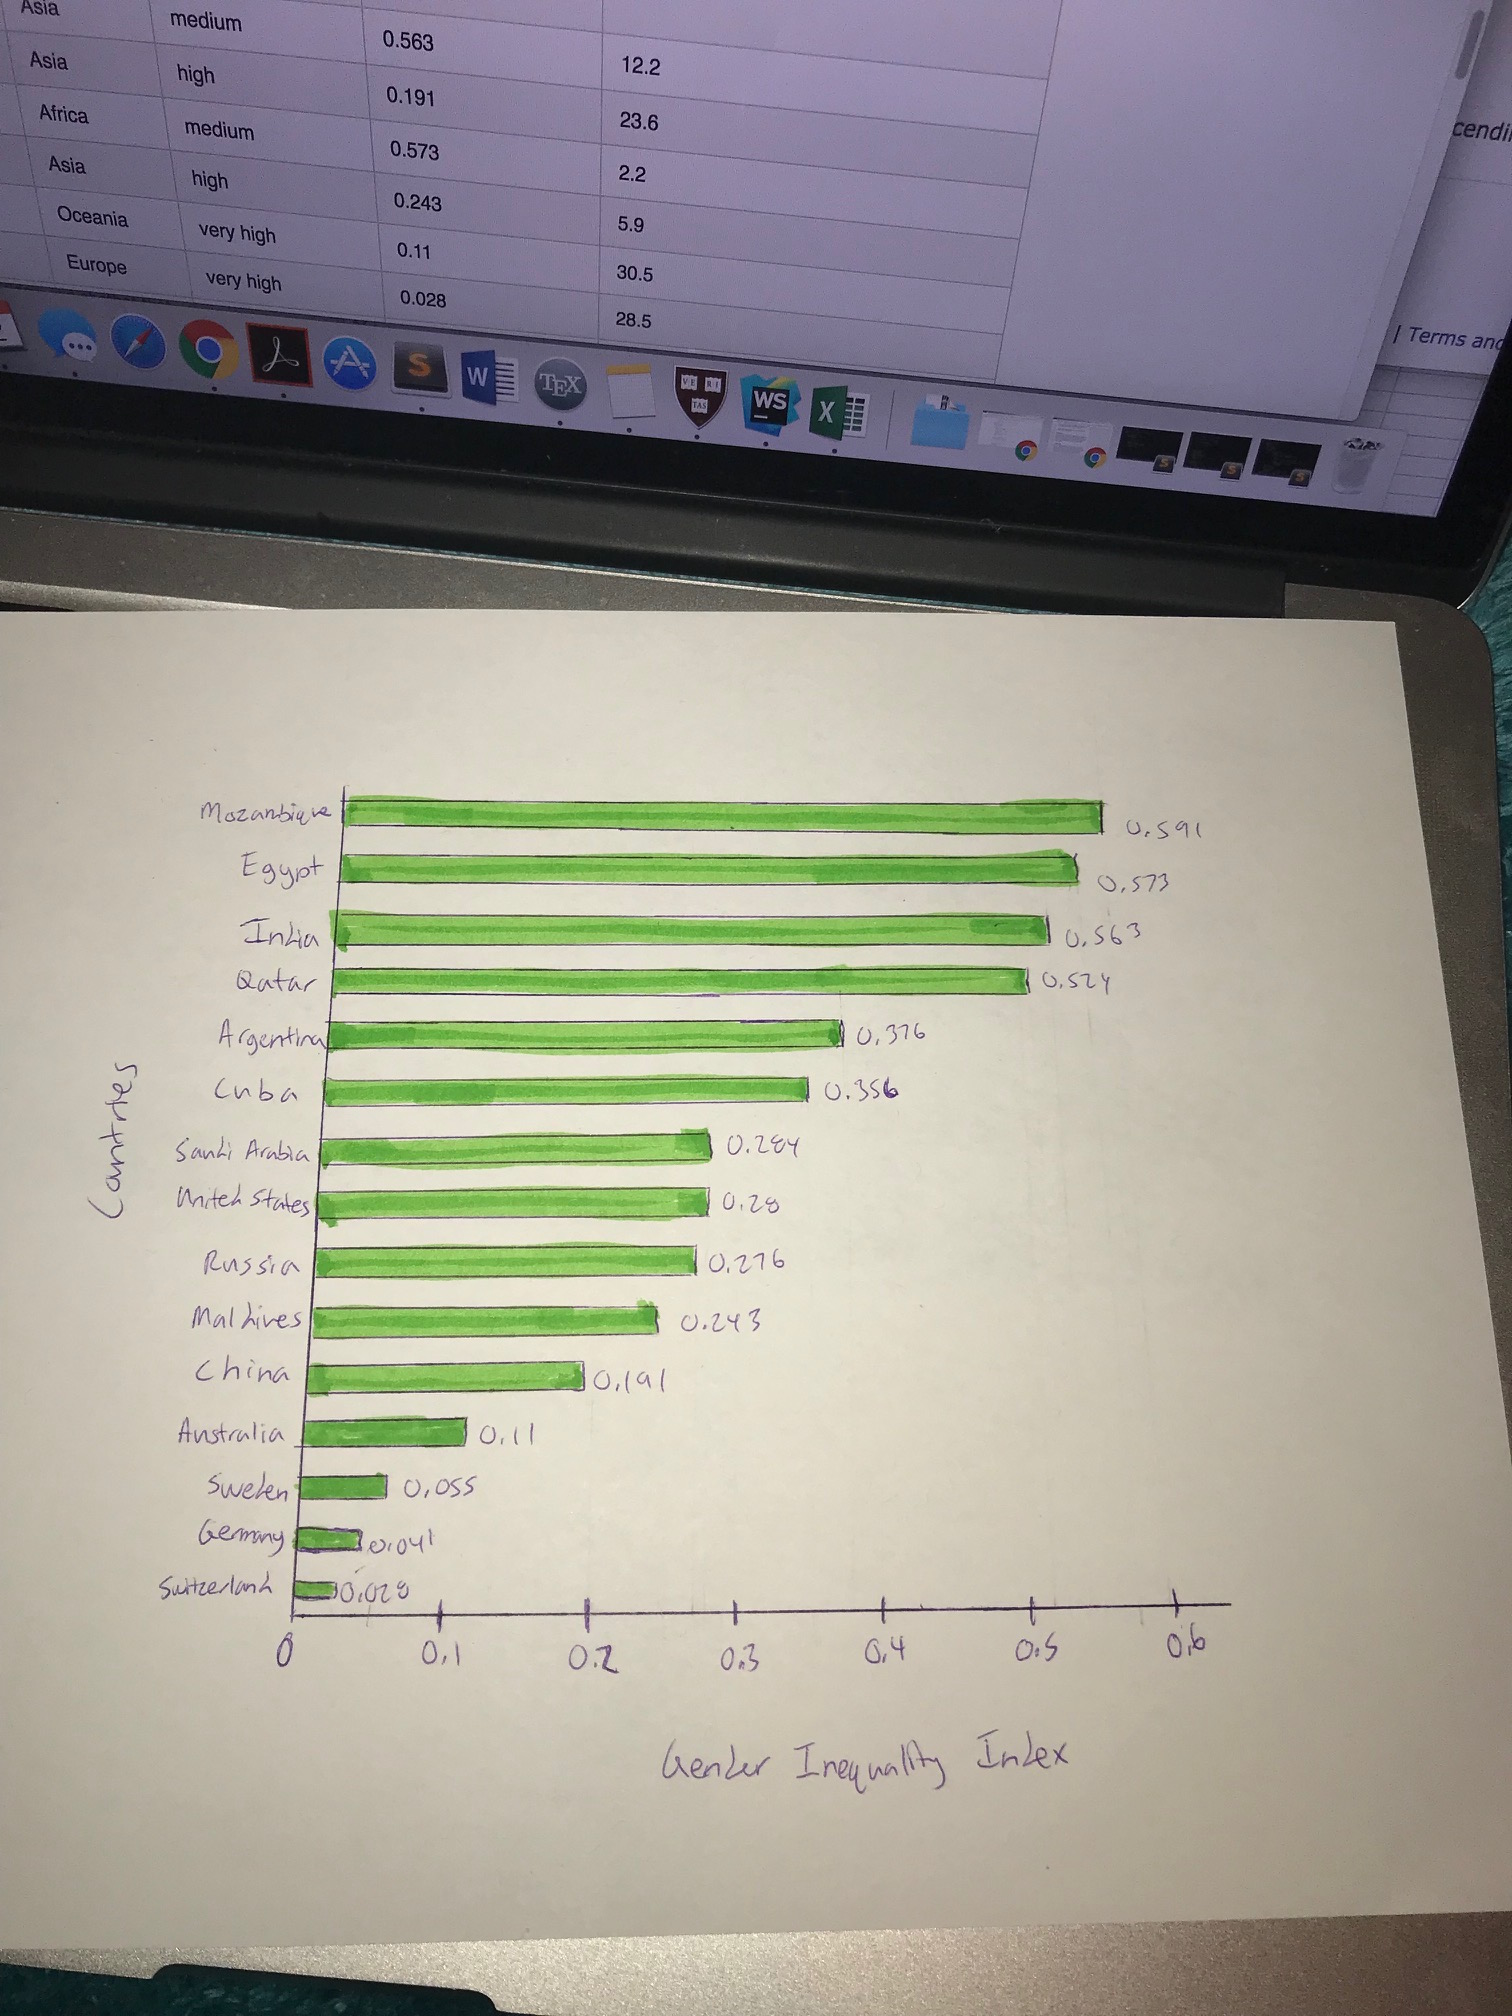
\includegraphics[scale=0.15]{sketch1}
  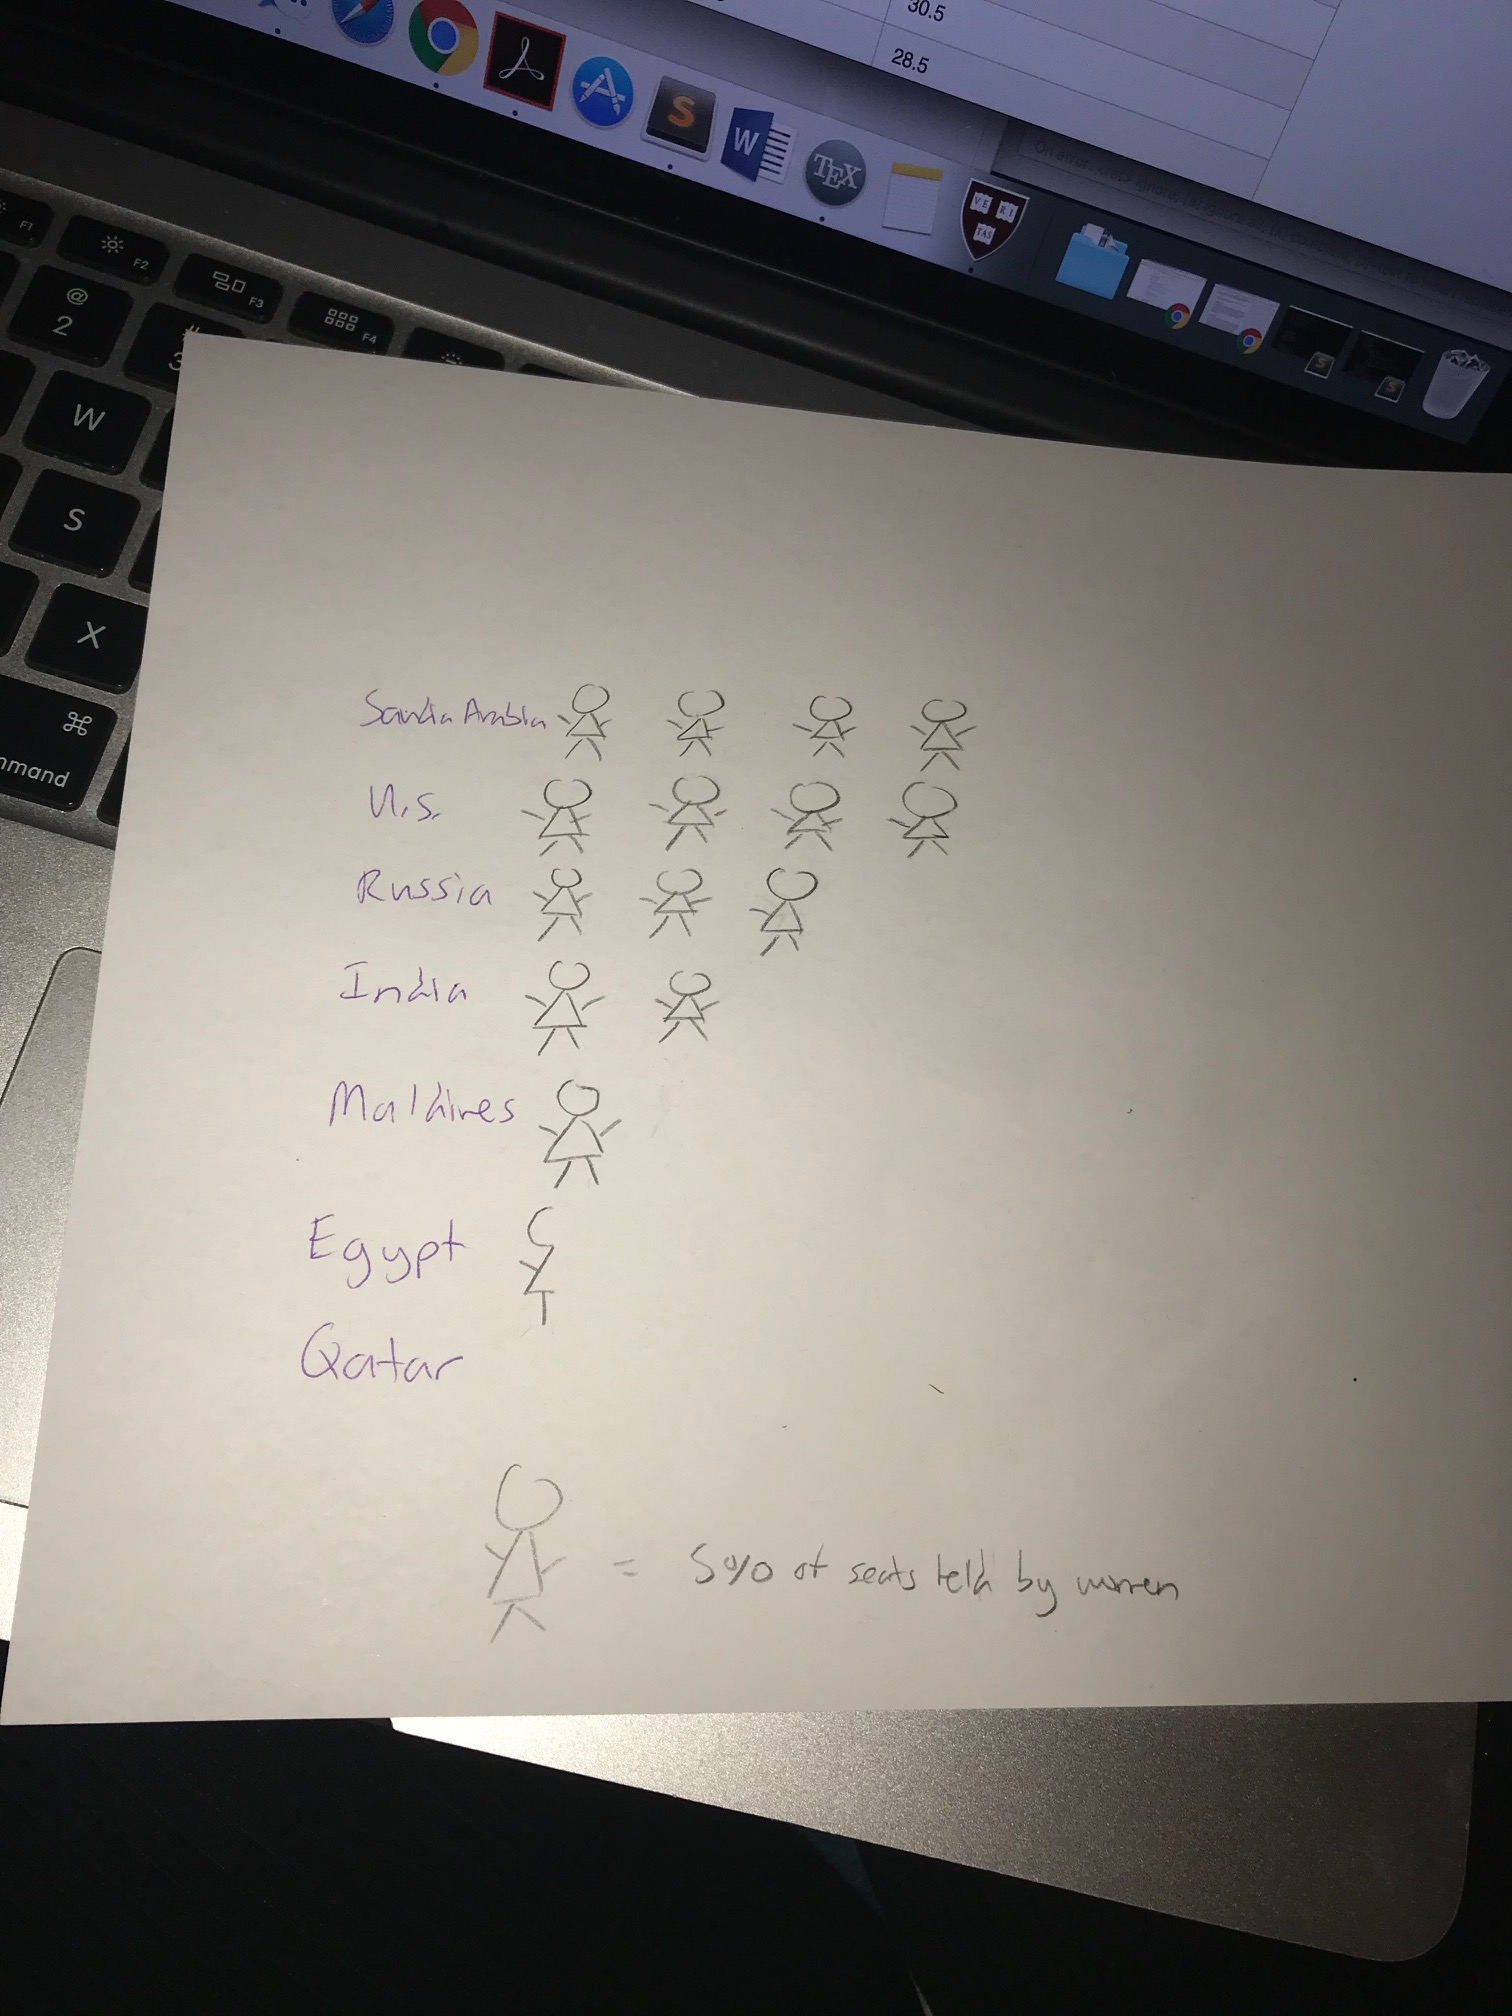
\includegraphics[scale=0.15]{sketch2}
  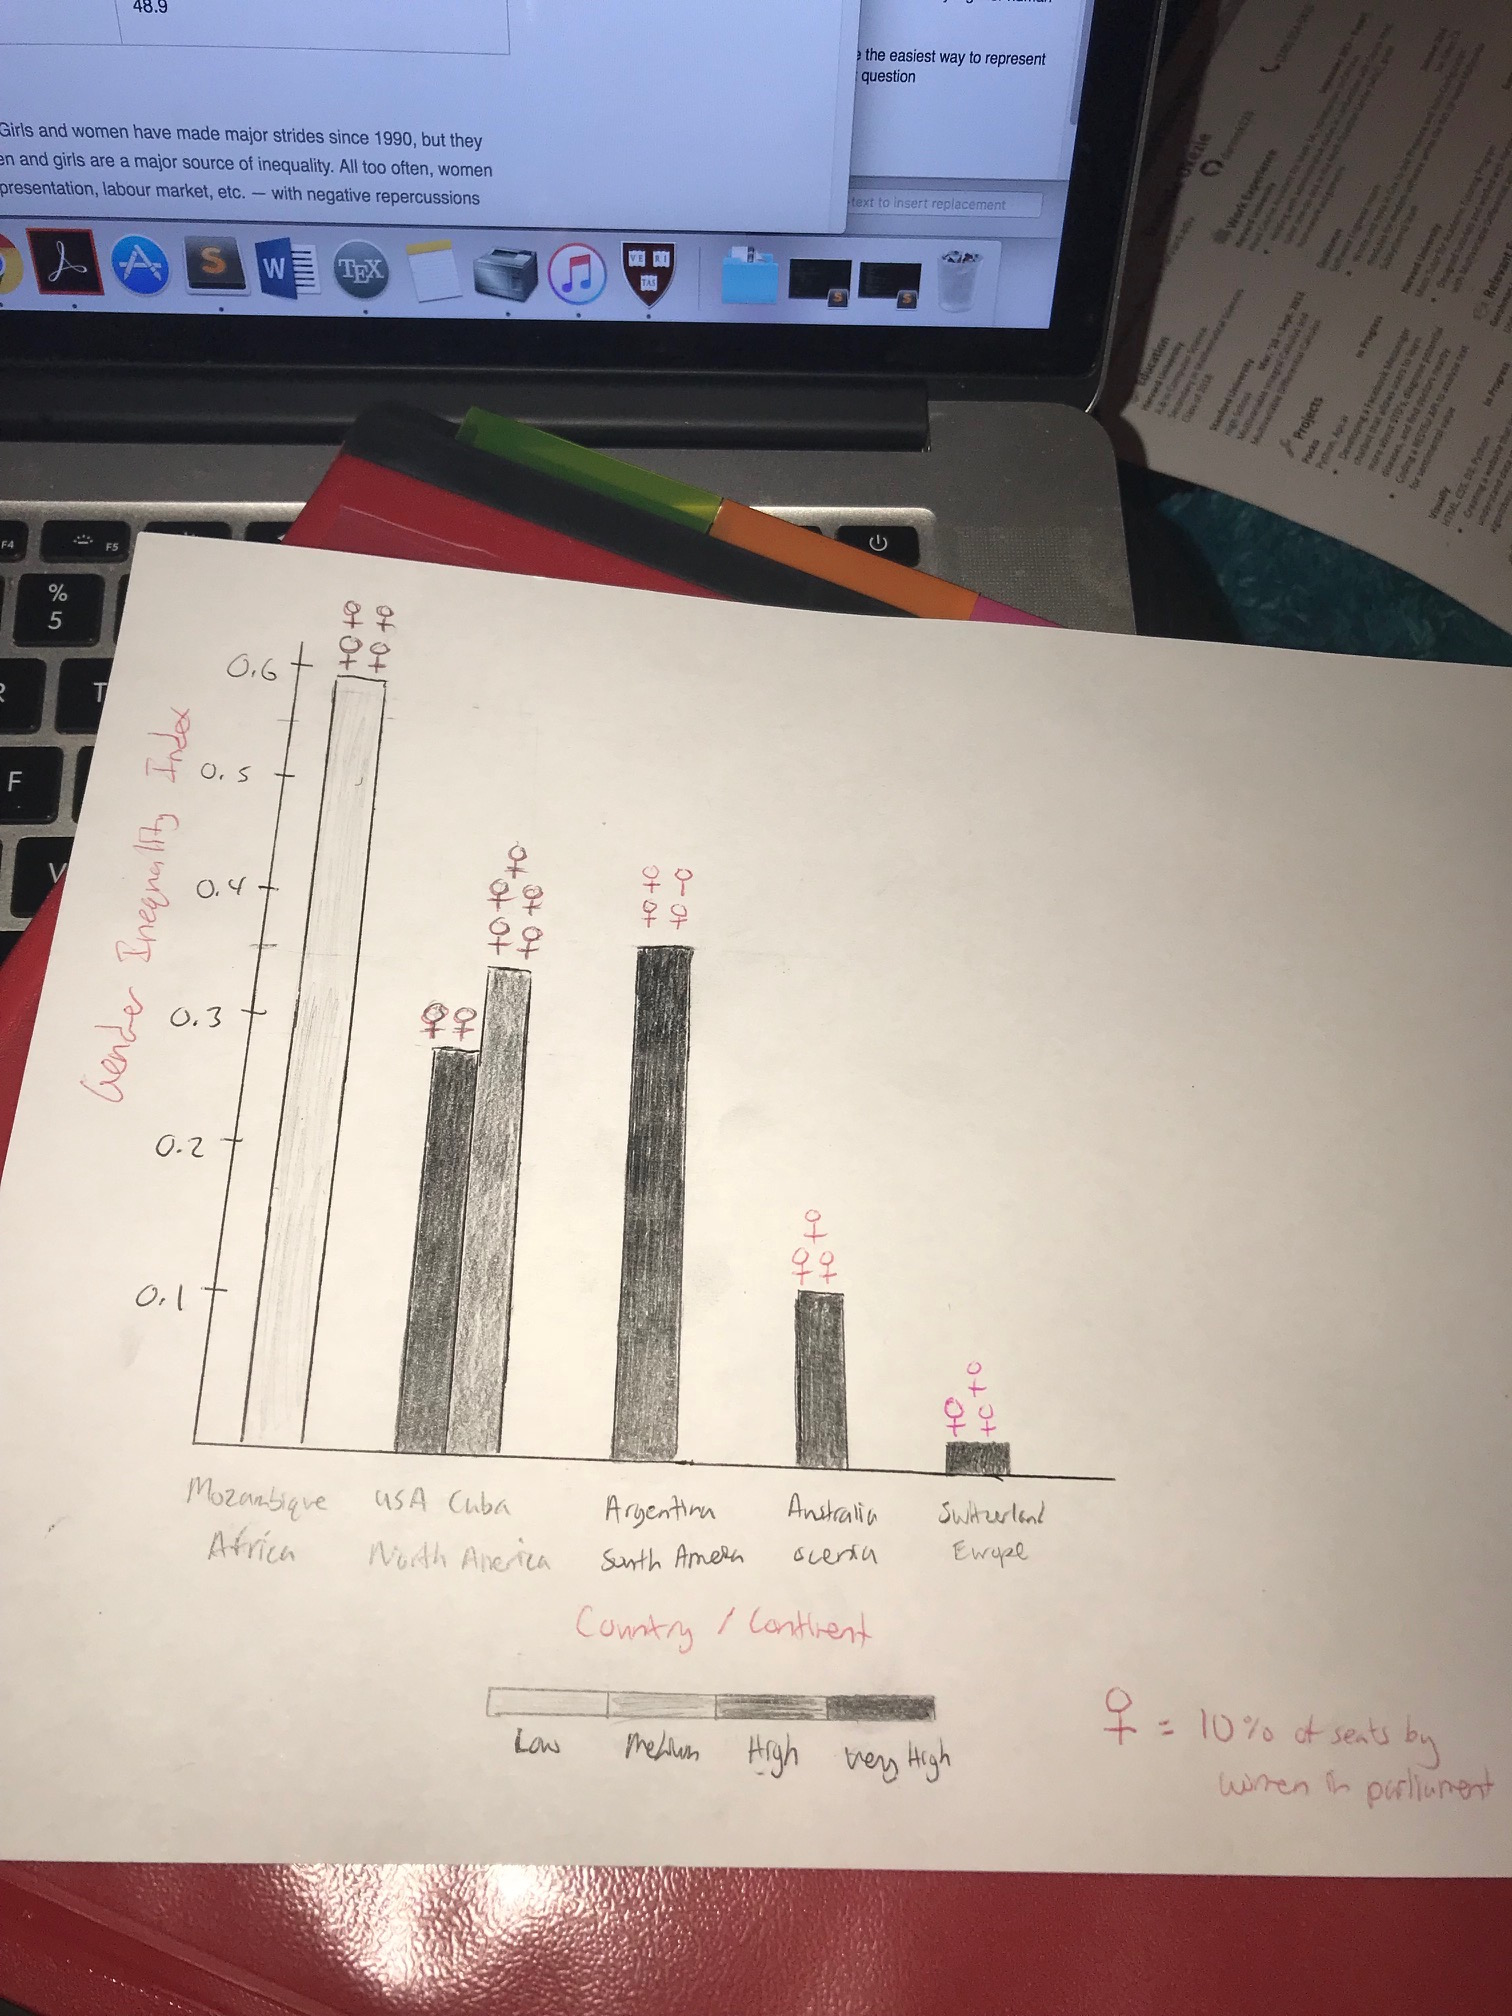
\includegraphics[scale=0.15]{sketch3}
  
  \item \textbf{Sketch 1}
  \begin{enumerate}
    \item I used color and position. Position as in ordering the countries in descending order by gender inequality index. 
    \item I didn't necessarily use any of Gestalt's principles for this sketch
    \item I was answering the first question. A person can easily point out that Switzerland has the lowest gender inequality index by looking at the lowest bar on the graph.
  \end{enumerate}
  
  \item \textbf{Sketch 2}
  \begin{enumerate}
    \item I used shape for my data. I was going to draw a chair to represent the percent of seats held by women but I can't draw chairs that well, so a stick figure woman was also another good choice.
    \item I used Gestalt's similarity principle.
    \item I am trying to answer the second question. I believe people read things in ascending order from bottom to up so it would make sense to put the lowest percent of seats help by women in parliament at the bottom, which is represented by Qatar.
  \end{enumerate}
  
  \item \textbf{Sketch 3}
  \begin{enumerate}
    \item I used grey value, shape, and size for my data. The grey value is used to represent the range from low to very high for human development. Shape is just a bar chart. Size is relative to the gender inequality index.
    \item I used Gestalt's similarity and proximity principle.
    \item I am trying to answer all three questions in the best way possible. I feel as though bar graphs are the easiest way to represent data for gender inequality data so I used that. For continent I just grouped it with the country.
  \end{enumerate}
  
  \item The person I peer reviewed is Jason Stein.
  
\end{enumerate}


\end{document}
